\documentclass[a4paper,11pt]{jsarticle}

% 数式
\usepackage{amsmath,amsfonts}
\usepackage{amsthm}
\usepackage{bm}
\usepackage{mathtools}
\usepackage{amssymb}

% 表
\usepackage[utf8]{inputenc}
\usepackage{diagbox} % 斜線付きセルを作成するために必要
\usepackage{booktabs} % 表の罫線を美しくするために必要
\usepackage{hhline} % 水平罫線を制御するために必要

% 画像
\usepackage[dvipdfmx]{graphicx}
\usepackage{ascmac}
\usepackage{physics}
\usepackage{float} % 追加

% 図
\usepackage[dvipdfmx]{graphicx}
\usepackage{tikz} %図を描く
\usetikzlibrary{positioning, intersections, calc, arrows.meta,math} %tikzのlibrary

% ハイパーリンク
\usepackage[dvipdfm,
  colorlinks=false,
  bookmarks=true,
  bookmarksnumbered=false,
  pdfborder={0 0 0},
  bookmarkstype=toc]{hyperref}

% 式番号を章ごとにリセット
\numberwithin{equation}{section}

\begin{document}

\title{情報幾何学の基礎}
\author{大上由人}
\date{\today}
\maketitle

\section[0]{はじめに}
\begin{itembox}[l]{\textbf{Thm:逆写像定理}}
点$\vb{a}=(a_1,\cdots,a_n)$を含む領域$D \subset \mathbb{R}^n$から$\mathbb{R}^n$への$C^1$級写像
\begin{equation}
    \vb{f} : D \to \mathbb{R}^n \quad \vb{x} =(x_1,\cdots,x_n) \mapsto \vb{y} =(f_1(\vb{x}),\cdots,f_n(\vb{x}))
\end{equation}
が、点$\vb{f(a)}$の近傍で$C^1$級の逆写像を持つための必要十分条件は、$\vb{f}$のヤコビ行列$\vb{J}(\vb{x})$が点$\vb{a}$で正則であることである。

\end{itembox}
\section{多様体のアフィン接続}
\subsection{ベクトル場の共変微分}
一般の多様体上では、共変微分を用いて平行移動を定義する。以下では初めに共変微分の定義を述べる。

\begin{itembox}[l]{\textbf{Def:共変微分}}
    Mを多様体とする。以下の4条件を満たす写像
    \begin{equation}
        \nabla : \mathfrak{X}(M) \times \mathfrak{X}(M) \to \mathfrak{X}(M) \quad (X,Y) \mapsto \nabla_XY
    \end{equation}
    をM上の共変微分という。
    \begin{enumerate}
        \item 
        \begin{equation}
            \nabla_X(Y+Z) = \nabla_XY + \nabla_XZ
        \end{equation}

        \item
        \begin{equation}
            \nabla_X(fY) = (Xf)Y + f\nabla_XY
        \end{equation}

        \item
        \begin{equation}
            \nabla_{X+Y}Z = \nabla_XZ + \nabla_YZ
        \end{equation}

        \item
        \begin{equation}
            \nabla_{fX}Y = f\nabla_XY
        \end{equation}
    \end{enumerate}
\end{itembox}
\textbf{ex:Euclid空間}\\
%時間がある時に書く

このとき、共変微分$\nabla_XY$は、テンソル性を満たさないが、これらの差はテンソル性を持つ。\\
$\because$\\
\begin{align}
    S(X,Y) &= \nabla_XY - \nabla'_{X}Y\\
\end{align}
に対して、任意の$f,g \in C^\infty(M)$に対して、
\begin{align}
    S(fX,gY) &= \nabla_{fX}(gY) - \nabla'_{fX}(gY)\\
    &= f\nabla_X(gY) - f\nabla'_{X}(gY)\\
    &= f((Xg)Y + g\nabla_XY) - f((Xg)Y + g\nabla'_{X}Y)\\
    &= fg\nabla_XY - fg\nabla'_{X}Y\\
    &= fgS(X,Y)
\end{align}
が成り立つ。\hfill\qedsymbol
したがって、$S$は$(1,2)$型のテンソル場である。したがって、$M$上に何か一つ共変微分を固定して、それとの差を考えると、$M$上の共変微分全体と、$(1,2)$型のテンソル場全体は、同型である。すなわち、
\begin{equation}
 \{\text{M上の共変微分全体}\} \simeq \nabla^{0} +\{\text{(1,2)型のテンソル場全体}\}
\end{equation}
となる。\\

次に、共変微分の局所座標表示を考える。
\begin{itembox}[l]{\textbf{Def:接続係数}}
    多様体$M$の座標近傍$(U;x^1,\cdots,x^n)$において、
    \begin{equation}
        \nabla_{\pdv{x^i}}\pdv{x^j} = \Gamma_{ij}^k\pdv{x^k}
    \end{equation}
    によって定義される、$n^3$個の関数$\Gamma_{ij}^k$を接続係数という。
\end{itembox}
これは、局所座標の取り方に依存することに注意する。別の座標近傍でも同様に、
\begin{equation}
    \nabla_{\pdv{\xi^a}}\pdv{\xi^b} = \Gamma_{ab}^c\pdv{\xi^c}
\end{equation}
により、接続係数の組$\{\Gamma_{ab}^c\}$が定義される。このとき、座標変換則を考える。
\begin{itembox}[l]{\textbf{Prop:接続係数の座標変換}}
    接続係数$\Gamma_{ij}^k$と$\Gamma_{ab}^c$の間には、次の関係が成り立つ。
    \begin{equation}
        \Gamma_{ij}^k = \pdv{\xi^a}{x^i}\pdv{\xi^b}{x^j}\pdv{x^k}{\xi^c}\Gamma_{ab}^c + \pdv[2]{\xi^c}{x^i}{x^j}\pdv{x^k}{\xi^c}
    \end{equation}
\end{itembox}
\textbf{Prf}\\
\begin{align}
    \nabla_{\pdv{x^i}}\pdv{x^j} &= \Gamma_{ij}^k\pdv{x^k}\\
    &= \Gamma_{ij}^k\pdv{\xi^c}{x^k}\pdv{\xi^c}\\
\end{align}
である、一方、
\begin{align}
    \nabla_{\pdv{x^i}}\pdv{x^j} &= \nabla_{\pdv{\xi^b}}\pdv{\xi^b}\\
    &= \pdv[2]{\xi^b}{x^i}{x^j}\pdv{\xi^b} + \pdv{\xi^b}{x^j}\nabla_{\pdv{x^i}}\pdv{\xi^b}\\
    &= \pdv[2]{\xi^b}{x^i}{x^j}\pdv{\xi^b} + \pdv{\xi^b}{x^j}\nabla_{(\pdv{\xi^a}{x^i}\pdv{xi^a})}\pdv{\xi^b}\\
    &= \pdv[2]{\xi^b}{x^i}{x^j}\pdv{\xi^b} + \pdv{\xi^b}{x^j}\pdv{\xi^a}{x^i}\nabla_{\pdv{\xi^a}}\pdv{\xi^b}\\
    &= \pdv[2]{\xi^b}{x^i}{x^j}\pdv{\xi^b} + \pdv{\xi^b}{x^j}\pdv{\xi^a}{x^i}\Gamma_{ab}^c\pdv{\xi^c}\\
    &= \pdv[2]{\xi^c}{x^i}{x^j}\pdv{\xi^c} + \pdv{\xi^b}{x^j}\pdv{\xi^a}{x^i}\Gamma_{ab}^c\pdv{\xi^c}\\
    &=(\pdv[2]{\xi^c}{x^i}{x^j} + \pdv{\xi^a}{x^i}\pdv{\xi^b}{x^j}\Gamma_{ab}^c)\pdv{\xi^c}
\end{align}
であるから、
\begin{equation}
    \Gamma_{ij}^k \pdv{\xi^c}{x^k} = \pdv[2]{\xi^c}{x^i}{x^j} + \pdv{\xi^a}{x^i}\pdv{\xi^b}{x^j}\Gamma_{ab}^c
\end{equation}
が成り立つ。したがって、
\begin{equation}
    \Gamma_{ij}^k = \pdv{\xi^a}{x^i}\pdv{\xi^b}{x^j}\pdv{x^k}{\xi^c}\Gamma_{ab}^c + \pdv[2]{\xi^c}{x^i}{x^j}\pdv{x^k}{\xi^c}
\end{equation}
が成り立つ。\hfill\qedsymbol

ところで、共変微分がテンソル性を満たさないことは上の座標変換の第二項が現れることによっても分かる。

\subsection{アフィン接続}
\begin{itembox}[l]{\textbf{Def:アフィン接続}}
    多様体$M$の各座標近傍に、上の座標変換則を満たすような$C^\infty(M)$上の関数の組$\{\Gamma_{ij}^k\}$を与えることを、$M$にアフィン接続を与えるといい、
    $\{\Gamma_{ij}^k\}$を接続係数という。
\end{itembox}
以下、アフィン接続を用いて、平行および平行移動を定義する。
\begin{itembox}[l]{\textbf{Def:平行}}
    多様体$M$にアフィン接続が与えられているとする。$M$上のなめらかな曲線
    \begin{equation}
        C = \{p(t) ; t \in [a,b]\}
    \end{equation}
    に沿って定義されたベクトル場$Z=\{Z_{p(t)}\}$が、$C$に沿って平行であるとは、
    \begin{equation}
        \nabla_{\dot{p}(t)}Z_{p(t)} = 0
    \end{equation}
    が成り立つことをいう。ここで、
    \begin{equation}
        \dot{p}(t) = \dv{x^i}{t}\pdv{x^i}
    \end{equation}
    である。
\end{itembox}
\textbf{Prf}\\
上の平行条件を局所座標表示する。
\begin{equation}
    Z_{p(t)} = Z^i\pdv{x^i}
\end{equation}
と成分表示すると、
\begin{align}
    \nabla_{\dot{p}(t)}Z &= \nabla_{\dv{x^i}{t} \pdv{x^i}} \left( Z^j \pdv{x^j} \right) \\
    &= \dv{x^i}{t} \left( \pdv{Z^j}{x^i} \pdv{x^j} + \dv{x^j}{t} Z^j \nabla_{\pdv{x^i}} \pdv{x^j} \right) \\
    &= \left( \dot{Z}^k + \dot{x}^i Z^j \Gamma_{ij}^k \right) \pdv{x^k}
\end{align}
となる。したがって、
\begin{equation}
    \label{eq:parallel_condition}
    \dot{Z}^k + \dot{x}^iZ^j\Gamma_{ij}^k = 0
\end{equation}
が成り立つ。

\textbf{ex:測地線}\\
%時間がある時に書く

\begin{itembox}[l]{\textbf{Def:平行移動}}
    多様体$M$上のなめらかな曲線$C = \{p(t) ; t \in [a,b]\}$と、$\vb{p} \in T_{p(a)}M$が任意に与えられたとき、\ref{eq:parallel_condition}
    の解として定まるベクトル場$Z$の$t=b$における値$Z_{p(b)}$を、$\vb{p}$を$t=a$から$t=b$に沿って平行移動して得られた接ベクトルという。\\
    また、この対応は全単射線形写像となり、\footnote{微分方程式の解の一意性から従う。}、
    \begin{equation}
        \label{eq:parallel_transport}
        \Pi_C : T_{p(a)}M \to T_{p(b)}M
    \end{equation}
    を定める。これを、曲線$C$に沿った平行移動という。
\end{itembox}
このとき、平行条件は、
\begin{equation}
    \vb{v} \in T_{p(a)}M \parallel \vb{w} \in T_{p(b)}M \Leftrightarrow \Pi_C \vb{v} = \vb{w}
\end{equation}
と書ける。\\

\begin{itembox}[l]{\textbf{Thm:共変微分の幾何的意味}}
    多様体$M$にアフィン接続が与えられているとし、点$p(a)\in M$を通るような$M$のなめらかな曲線
    \begin{equation}
        C = \{p(t) ; t \in [a-\epsilon,a+\epsilon]\}
    \end{equation}
    を考える。任意のベクトル場$Y \in \mathfrak{X}(M)$に対して、
    \begin{equation}
        (\nabla_{\dot{p}(t)} Y)_{p(a)} = \underset{t \to a}{\lim} \frac{1}{t-a}(\Pi_{p(a)}^{p(t)}Y_{p(t)} - Y_{p(a)})
    \end{equation}
    が成り立つ。ここで、$\Pi_{p(a)}^{p(t)}$は、$p(t)$から$p(a)$に沿って平行移動する写像である。
\end{itembox}
\textbf{Prf}\\
%TODO:証明を書く

\subsection{曲率}
平行移動が、経路に依存することを示すために、曲率を導入する。以降、$\pdv{x^i}$を$\partial{i}$と略記する。

\begin{itembox}[l]{\textbf{Def:曲率テンソル場}}
    多様体$M$にアフィン接続が与えられているとする。$M$上で定義された3重$C^\infty(M)$-テンソル場$R$を、
    \begin{align}
        R : &\mathfrak{X}(M) \times \mathfrak{X}(M) \times \mathfrak{X}(M) \to \mathfrak{X}(M) \\
        & (X,Y,Z) \mapsto \nabla_X(\nabla_YZ) - \nabla_Y(\nabla_XZ) - \nabla_{[X,Y]}Z
    \end{align}
    によって定義する。このテンソル場を、接続$\nabla$の曲率テンソル場という。

\end{itembox}
局所座標表示すると、
\begin{align}
    R(\partial_{i},\partial_{j},\partial_{k}) &= R_{ijk}^l\partial_{l}\\
\end{align}
となる。右辺を具体的に求めると、
%TODO:具体的な計算を書く
よって、
\begin{equation}
    R_{ijk}^l = \partial_{i}\Gamma_{jk}^l - \partial_{j}\Gamma_{ik}^l + \Gamma_{im}^l\Gamma_{jk}^m - \Gamma_{jm}^l\Gamma_{ik}^m
\end{equation}
となる。
%TODO:ここにも追記する。

\begin{itembox}[l]{\textbf{Prop:曲率と平行移動}}
    曲率が0であることと、平行移動が経路に依存しないことは同値である。
\end{itembox}
\textbf{Prf}\\
%TODO:証明を書く

\newpage
\subsection{捩率}
\begin{itembox}[l]{\textbf{Def:捩率}}
    アフィン接続$\nabla$をもつ多様体$M$上で定義された二重$C^\infty(M)$-テンソル場$T$を、
    \begin{align}
        T : &\mathfrak{X}(M) \times \mathfrak{X}(M) \to C^\infty(M) \\
        & (X,Y) \mapsto \nabla_XY - \nabla_YX - [X,Y]
    \end{align}
    によって定義する。このテンソル場を、接続$\nabla$の捩率テンソル場という。
\end{itembox}

このとき、\(T\) は \((1,2)\) 型テンソル場である。\\
$\because$ 共変微分の定義を繰り返し用いる。
\begin{align}
T(fX, gY) &= \nabla_{fX}(gY) - \nabla_{gY}(fX) - [fX, gY] \\
          &= f\nabla_X(gY) - g\nabla_Y(fX) \\
          &\quad - f(Xg)Y - fg(XY) + g(Yf)X + fg(YX) \\
          &= f(Xg)Y + fg\nabla_X Y - f(Yf)X - fg\nabla_Y X \\
          &\quad - f(Xg)Y - fg(XY) + g(Yf)X + fg(YX) \\
          &= fg(\nabla_X Y - \nabla_Y X - [X, Y]) \\
          &= fgT(X, Y)
\end{align}

となり、\((1,2)\) 型テンソル場であることがわかる。\hfill\qedsymbol

局所座標表示すると、
\begin{align}
    T(\partial_{i},\partial_{j}) &= T_{ij}^k\partial_{k}\\
\end{align}
と定義される。$T_{ij}^k$を具体的に求める。左辺について、
\begin{align}
    T(\partial_{i},\partial_{j}) &= \nabla_{\partial_{i}}\partial_{j} - \nabla_{\partial_{j}}\partial_{i} - [\partial_{i},\partial_{j}]\\
    &= \nabla_{\partial_{i}}\partial_{j} - \nabla_{\partial_{j}}\partial_{i} - 0\\
    &= \Gamma_{ij}^k\partial_{k} - \Gamma_{ji}^k\partial_{k}\\
    &= (\Gamma_{ij}^k - \Gamma_{ji}^k)\partial_{k}
\end{align}
となるから、
\begin{equation}
    T_{ij}^k = \Gamma_{ij}^k - \Gamma_{ji}^k
\end{equation}
となる。\\
捩率の幾何的な意味を見るために、曲率のときと同様に、微小四辺形をに沿って接ベクトルを平行移動してみる。

\begin{align}
    \label{eq:torsion_condition}
    \{\epsilon_i \partial_{i}(x)+\epsilon_j\Pi_{x}^{x+\delta_i}\partial_{j}(x+\delta_i)\} - \{\epsilon_j \partial_{j}(x)+\epsilon_i\Pi_{x}^{x+\delta_j}\partial_{i}(x+\delta_j)\} 
\end{align}
について考える。これは、それぞれ、i方向への微小変化の後にj方向に微小変化させることと、j方向への微小変化の後にi方向に微小変化させることを表している。まず、
\begin{equation}
    \Pi_{x}^{x+\delta_i}\partial_{j}(x+\delta_i) = \partial_{j}(x)+\epsilon_i \Gamma_{ij}^k\partial_{k}+\mathcal{O}(\epsilon_i^2)
\end{equation}
であるから、
\begin{align}
    \epsilon_i \partial_{i}(x)+\epsilon_j\Pi_{x}^{x+\delta_i}\partial_{j}(x+\delta_i) &= \epsilon_i \partial_{i}(x)+\epsilon_j(\partial_{j}(x)+\epsilon_i \Gamma_{ij}^k\partial_{k})+\mathcal{O}(\epsilon_i^2)\\
    &= \epsilon_i \partial_{i}(x)+\epsilon_j\partial_{j}(x)+\epsilon_j\epsilon_i \Gamma_{ij}^k\partial_{k}+\mathcal{O}(\epsilon_i^2)
\end{align}
となる。同様に、
\begin{align}
    \epsilon_j \partial_{j}(x)+\epsilon_i\Pi_{x}^{x+\delta_j}\partial_{i}(x+\delta_j) &= \epsilon_j \partial_{j}(x)+\epsilon_i(\partial_{i}(x)+\epsilon_j \Gamma_{ji}^k\partial_{k})+\mathcal{O}(\epsilon_j^2)\\
    &= \epsilon_j \partial_{j}(x)+\epsilon_i\partial_{i}(x)+\epsilon_i\epsilon_j \Gamma_{ji}^k\partial_{k}+\mathcal{O}(\epsilon_j^2)
\end{align}
となる。したがって、(\ref{eq:torsion_condition})は、
\begin{align}
    \epsilon_j\epsilon_i \Gamma_{ij}^k\partial_{k} - \epsilon_i\epsilon_j \Gamma_{ji}^k\partial_{k}=\epsilon_j\epsilon_i T_{ij}^k\partial_{k}
\end{align}
となる。すなわち、捩率は、ベクトルの和の経路依存性の、面積要素の比例する主要部分を表している。\\

\subsection{平坦な多様体とアフィン座標系}
\begin{itembox}[l]{\textbf{Def:$\nabla$-平坦}}
    多様体$M$にアフィン接続$\nabla$が与えられているとする。このとき、$\nabla$が平坦であるとは、$R$と$T$が恒等的に0であることをいう。
\end{itembox}

\begin{itembox}[l]{\textbf{Def:$\nabla$-アフィン座標系}}
    多様体$M$にアフィン接続$\nabla$が与えられているとする。$M$の座標近傍$(U;x^1,\cdots,x^n)$において、接続係数$\{\Gamma_{ij}^k\}$がすべて恒等的に0であるとき、
    この座標近傍を$\nabla$-アフィン座標近傍といい、局所座標系$(x^i)$を$\nabla$-アフィン座標系という。
\end{itembox}

\textbf{Rem}\\
平坦であるという性質は(曲率や捩率がテンソルで定義されているのだから)座標の取り方に依らないが、アフィン座標系かどうかは座標の取り方に依存する。\\\\

\begin{itembox}[l]{\textbf{Thm:局所アフィン座標系の存在}}
    多様体$M$にアフィン接続$\nabla$が与えられているとする。このとき、以下の二つは同値である。
    \begin{enumerate}
        \item $M$は、$\nabla$-平坦である。
        \item $M$の任意の点$p \in M$において、$\nabla$-アフィン座標近傍が存在する。
    \end{enumerate}
\end{itembox}
\textbf{Prf}\\
(2) $\Rightarrow$ (1)\\
接続係数が恒等的に0となる局所座標系があったならば、曲率と捩率の定義より、その座標系での曲率と捩率は0である。また、曲率と捩率はテンソル場であるから、それは座標系に依らない。したがって、$\nabla$は平坦である。\\
(1) $\Rightarrow$ (2)\\
任意の座標近傍$(U;x^1,\cdots,x^n)$に対して、ある座標近傍$(V;\xi^1,\cdots,\xi^n)$が存在して、$U \cap V$で、
\begin{equation}
    \label{eq:affine_coordinate}
    0=\Gamma_{ab}^c = \pdv{x^i}{\xi^a}\pdv{x^j}{\xi^b}\pdv{\xi^c}{x^k}\Gamma_{ij}^k + \pdv[2]{x^l}{\xi^a}{\xi^b}\pdv{\xi^c}{x^l} \quad \forall a,b,c
\end{equation}
が成り立つことを示す。\\

\begin{equation}
    \frac{\partial x^\ell}{\partial \xi^b} \frac{\partial \xi^b}{\partial x^j} = \delta^\ell_j
    \end{equation}
    
    の両辺を $x^i$ で偏微分して
    \begin{equation}
    \frac{\partial^2 x^\ell}{\partial \xi^a \partial \xi^b} \frac{\partial \xi^a}{\partial x^i} \frac{\partial \xi^b}{\partial x^j} + \frac{\partial x^\ell}{\partial \xi^b} \frac{\partial^2 \xi^b}{\partial x^i \partial x^j} = 0
    \end{equation}
    
    だから,両辺に Jacobi 行列 $\frac{\partial \xi^a}{\partial x^i}$ と $\frac{\partial \xi^b}{\partial x^j}$ の逆行列を掛けて
    \begin{equation}
    \frac{\partial^2 x^\ell}{\partial \xi^a \partial \xi^b} = -\frac{\partial x^i}{\partial \xi^a} \frac{\partial x^j}{\partial \xi^b} \frac{\partial x^\ell}{\partial \xi^d} \frac{\partial^2 \xi^d}{\partial x^i \partial x^j}
    \end{equation}
    
    この式を (\ref{eq:affine_coordinate}) に代入して
    \begin{align}
    0 &= \frac{\partial x^i}{\partial \xi^a} \frac{\partial x^j}{\partial \xi^b} \frac{\partial \xi^c}{\partial x^k} \Gamma^k_{ij} - \left( \frac{\partial x^i}{\partial \xi^a} \frac{\partial x^j}{\partial \xi^b} \frac{\partial x^\ell}{\partial \xi^d} \frac{\partial^2 \xi^d}{\partial x^i \partial x^j} \right) \frac{\partial \xi^c}{\partial x^\ell} \\
    &= \frac{\partial x^i}{\partial \xi^a} \frac{\partial x^j}{\partial \xi^b} \frac{\partial \xi^c}{\partial x^k} \Gamma^k_{ij} - \frac{\partial x^i}{\partial \xi^a} \frac{\partial x^j}{\partial \xi^b} \delta^d \frac{\partial^2 \xi^d}{\partial x^i \partial x^j} \\
    &= \frac{\partial x^i}{\partial \xi^a} \frac{\partial x^j}{\partial \xi^b} \left( \frac{\partial \xi^c}{\partial x^k} \Gamma^k_{ij} - \frac{\partial^2 \xi^c}{\partial x^i \partial x^j} \right)
    \end{align}
    
    従って、(\ref{eq:affine_coordinate}) は次式と同値である。
    \begin{equation}
    \frac{\partial^2 \xi^c}{\partial x^i \partial x^j} = \frac{\partial \xi^c}{\partial x^k} \Gamma^k_{ij}
    \end{equation}
    
    あるいはこれを連立方程式の形で書けば
    \begin{align}
        \frac{\partial \xi^c}{\partial x^k} &= \theta^c_k \\
        \pdv{\xi^c}{x^i}{x^j} &= \theta^c_k \Gamma^k_{ij}
    \end{align}

この連立偏微分方程式の可積分条件は
    \begin{align}
        \pdv[2]{\xi^c}{x^i}{x^j} &= \pdv[2]{\xi^c}{x^j}{x^i} \\
        \pdv[2]{\theta^c_i}{x^i}{x^j} &= \pdv[2]{\theta^c_k}{x^j}{x^i}
    \end{align}
となる。これの第1式を同値変形していくと、
\begin{equation}
    \frac{\partial^2 \xi^c}{\partial x^i \partial x^j} = \frac{\partial^2 \xi^c}{\partial x^j \partial x^i}
\end{equation}
\begin{equation}
    \Leftrightarrow \frac{\partial}{\partial x^i} \theta^c_j = \frac{\partial}{\partial x^j} \theta^c_i
\end{equation}
\begin{equation}
    \Leftrightarrow \theta^c_k \Gamma^k_{ij} = \theta^c_k \Gamma^k_{ji}
\end{equation}
\begin{equation}
    \Leftrightarrow \theta^c_k T^k_{ij} = 0
\end{equation}
同様に、第2式を同値変形していくと、
\begin{equation}
    \frac{\partial^2 \theta^c_k}{\partial x^i \partial x^j} = \frac{\partial^2 \theta^c_k}{\partial x^j \partial x^i} \iff \frac{\partial}{\partial x^i} (\theta^c_l \Gamma^l_{jk}) = \frac{\partial}{\partial x^j} (\theta^c_l \Gamma^l_{ik})
\end{equation}

\begin{equation}
    \iff (\theta^c_m \Gamma^m_{il}) \Gamma^l_{jk} + \theta^c_l \left( \partial_i \Gamma^l_{jk} \right) = (\theta^c_m \Gamma^m_{jl}) \Gamma^l_{ik} + \theta^c_l \left( \partial_j \Gamma^l_{ik} \right)
\end{equation}

\begin{equation}
    \iff \theta^c_m \left\{ \Gamma^m_{il} \Gamma^l_{jk} + \partial_i \Gamma^m_{jk} - \Gamma^m_{jl} \Gamma^l_{ik} - \partial_j \Gamma^m_{ik} \right\} = 0
\end{equation}

\begin{equation}
    \iff \theta^c_m R^m_{ijk} = 0
\end{equation}

さて,仮定より \(T = 0\) かつ \(R = 0\) であるから,連立微分方程式 (3.22) は可積分であることが分かる。
%TODO:続きを書く
まとめると、任意に固定した$p \in U$における初期条件$\psi(p)=(\xi^c)_p,(Jf)_p=(\partial_i \xi^c)_p$を二にに与えると、これを満たすような偏微分方程式の解$\xi^c$が局所的に存在する。\\
したがって、特に初期条件を$\det(Jf)_p\neq 0$とすると、$\xi^c$は$p$の近傍で局所座標系を張る。したがって、$\nabla$-アフィン座標系が存在する。\hfill\qedsymbol

\begin{itembox}[l]{\textbf{Thm:アフィン座標系の自由度}}
    多様体$M$に座標近傍$(U;x^i)$と$(V;\xi^a)$が与えられていて、$(x^i)$が局所$\nabla$-アフィン座標系であるとする。このとき、
    \begin{equation}
        (V;\xi^a)\text{が局所$\nabla$-アフィン座標系である} \Leftrightarrow \exists A \in GL(n,\mathbb{R}) \text{ s.t. } \xi^i = A^i_jx^j + b_i
    \end{equation}
    が成り立つ。ここで、$GL(n,\mathbb{R})$は$n$次正則行列全体の集合であり、$b_i$は定数である。
\end{itembox}
\textbf{Prf}\\
接続係数の座標変換則:
\begin{equation}
    \Gamma^k_{ij} = \frac{\partial \xi^a}{\partial x^i} \frac{\partial \xi^b}{\partial x^j} \frac{\partial x^k}{\partial \xi^c} \Gamma^c_{ab} + \frac{\partial^2 \xi^c}{\partial x^i \partial x^j} \frac{\partial x^k}{\partial \xi^c}
\end{equation}

において、\(\Gamma^k_{ij} = 0\) であるという条件のもとで \(\Gamma^c_{ab} = 0\) となるための必要十分条件は、第二項が消えることである。すなわち、
\begin{equation}
    \frac{\partial^2 \xi^c}{\partial x^i \partial x^j} = 0
\end{equation}

であり、これは示すべき式と同値である。またこのとき、\(A\) は座標変換の Jacobi 行列なので、特に正則となる。\hfill\qedsymbol
%TODO:最後だけ怪しい

\subsection{Riemann接続}
\begin{itembox}[l]{\textbf{Def:Riemann多様体}}
    $M$上で定義された(0,2)型テンソル場$g$であって、各点$p \in M$で、$g_p$が内積を定めるとき、$g$を$M$上のRiemann計量という。このとき、$(M,g)$をRiemann多様体という。
    ここで、
    \begin{equation}
        g_{ij} = g(\partial{i},\partial{j})
    \end{equation}
    は正定値対称行列となる。
\end{itembox}


\begin{itembox}[l]{\textbf{Def:Riemann接続/Levi-Civita接続/Levi-Civita平行移動}}
    Riemann多様体$(M,g)$の各座標近傍$(U;x^1,\cdots,x^n)$において、
    \begin{equation}
        \Gamma_{ij,k} = \Gamma_{ij}^l g_{lk}=\frac{1}{2}(\partial_i g_{jk} + \partial_j g_{ki} - \partial_k g_{ij})
    \end{equation}
    により定まる$M$のアフィン接続を、Levi-Civita接続という。また、この接続が定める$M$上の平行移動をLevi-Civita平行移動という。  

\end{itembox}

このとき、Levi-Civita接続はaffine接続を定める。\\
$\because$\\
計量
\begin{equation}
    g_{ij} = g(\partial_i,\partial_j)
\end{equation}
の座標変換は、
\[
\begin{aligned}
g_{ik} &= \frac{\partial x^b}{\partial x^i} \frac{\partial x^c}{\partial x^k} g_{bc}, \\
g_{ki} &= \frac{\partial x^c}{\partial x^k} \frac{\partial x^a}{\partial x^i} g_{ca}, \\
g_{ij} &= \frac{\partial x^a}{\partial x^i} \frac{\partial x^b}{\partial x^j} g_{ab},
\end{aligned}
\]
で与えられる。そして、
\begin{align}
\begin{aligned}
\partial_i g_{ik} &= \pdv{\xi^b}{x^j} \pdv{\xi^c}{x^k} \pdv{\xi^l}{x^i} \pdv{g_{bc}}{\xi^l} + g_{bc} \partial_i \left( \pdv{\xi^b}{x^j} \pdv{\xi^c}{x^k} \right), \\
\partial_j g_{ki} &= \pdv{\xi^c}{x^k} \pdv{\xi^a}{x^i} \pdv{\xi^l}{x^j} \pdv{g_{ca}}{\xi^l} + g_{ca} \partial_j \left( \pdv{\xi^c}{x^k} \pdv{\xi^a}{x^i} \right), \\
\partial_k g_{ij} &= \pdv{\xi^a}{x^i} \pdv{\xi^b}{x^j} \pdv{\xi^l}{x^k} \pdv{g_{ab}}{\xi^l} + g_{ab} \partial_k \left( \pdv{\xi^a}{x^i} \pdv{\xi^b}{x^j} \right),
\end{aligned}
\end{align}
であるから、
\begin{align}
    \Gamma_{ij,k} &= \frac{1}{2} \left( \partial_i g_{jk} + \partial_j g_{ki} - \partial_k g_{ij} \right) \\
    &= \frac{1}{2} \left[ \pdv{\xi^a}{x^i} \pdv{\xi^b}{x^j} \pdv{\xi^c}{x^k} \left( \pdv{g_{bc}}{\xi^a} + \pdv{g_{ca}}{\xi^b} - \pdv{g_{ab}}{\xi^c} \right) \right. \\
    &\quad + g_{bc} \left( \pdv[2]{\xi^b}{x^i}{x^j} \pdv{\xi^c}{x^k} + \pdv{\xi^b}{x^j} \pdv[2]{\xi^c}{x^k}{x^i} \right) \\
    &\quad + g_{ca} \left( \pdv[2]{\xi^c}{x^j}{x^k} \pdv{\xi^a}{x^i} + \pdv{\xi^c}{x^k} \pdv[2]{\xi^a}{x^i}{x^j} \right) \\
    &\quad - g_{ab} \left( \pdv[2]{\xi^a}{x^k}{x^i} \pdv{\xi^b}{x^j} + \pdv{\xi^a}{x^i} \pdv[2]{\xi^b}{x^j}{x^k} \right) \left. \right] \\
    &= \pdv{\xi^a}{x^i} \pdv{\xi^b}{x^j} \pdv{\xi^c}{x^k} \Gamma_{ab,c} + \pdv{\xi^c}{x^k} \pdv[2]{\xi^b}{x^i}{x^j} g_{bc}
\end{align}

となる。両辺に$g^{kl}=\pdv{x^k}{\xi^c}\pdv{x^l}{\xi^d}g^{cd}$をかけて縮約すると、
\begin{align}
    \Gamma_{ij}^l &= \pdv{\xi^a}{x^i} \pdv{\xi^b}{x^j} \pdv{\xi^c}{x^k} \Gamma_{ab,c}\pdv{x^k}{\xi^c}\pdv{x^l}{\xi^d}g^{cd}\\
    &\quad + \pdv{\xi^c}{x^k} \pdv[2]{\xi^b}{x^i}{x^j}g_{bc}\pdv{x^k}{\xi^c}\pdv{x^l}{\xi^d}g^{cd}\\
    &= \pdv{\xi^a}{x^i} \pdv{\xi^b}{x^j} \pdv{x^l}{\xi^d} \Gamma_{ab}^d + \pdv[2]{\xi^c}{x^i}{x^j}\pdv{x^l}{\xi^c}
\end{align}
となる。したがって、Levi-Civita接続の接続係数は、計量の座標変換則と同様に変換する。\hfill\qedsymbol

\begin{itembox}[l]{\textbf{Thm:平行移動に対する内積の不変性}}
    なめらかな曲線$C = \{p(t) ; t \in [a,b]\}$に沿ったLevi-Civita平行移動によって、内積は不変である。すなわち、
    \begin{equation}
        g_p(b)\left(\Pi_b^a \vb{v},\Pi_b^a \vb{w}\right) = g_p(a)(\vb{v},\vb{w})
    \end{equation}
    が成り立つ。
\end{itembox}
\textbf{Prf}\\
\begin{align}
    \frac{d}{dt} g_{p(t)} (Y_{p(t)}, Z_{p(t)}) &= 0 \\
\end{align}
であることを示せばよい。
\begin{align}
    \frac{d}{dt} g_{p(t)} (Y_{p(t)}, Z_{p(t)}) &= \frac{d}{dt} \left( Y^i(t) (\partial_i)_{p(t)}, Z^j(t) (\partial_j)_{p(t)} \right) \notag \\
    &= \frac{d}{dt} (Y^i Z^j g_{ij}) \\
    \text{∵} \quad \frac{d}{dt} g_{ij} &= \frac{dx^k}{dt} \partial_k g_{ij} \notag \\
    &= \left( \dot{Y}^i Z^j + Y^i \dot{Z}^j \right) g_{ij} + Y^i Z^j \partial_k g_{ij} \dot{x}^k \\
    \text{∵ 平行移動で} \quad \dot{Y}^i &= -\Gamma_{kl}^i \dot{x}^k Y^l, \quad \dot{Z}^j = -\Gamma_{kl}^j \dot{x}^k Z^l \\
    &= (\partial_k g_{ij} - \Gamma_{ki,j} - \Gamma_{kj,i}) \dot{x}^k Y^i Z^j \notag \\
    &=  \left( \right. \partial_k g_{ij}- \frac{1}{2} (\partial_k g_{ij} + \partial_i g_{jk} - \partial_j g_{ki}) \\
    &\quad - \frac{1}{2} (\partial_k g_{ji} + \partial_j g_{ik} - \partial_i g_{kj})\left.\right) \dot{x}^k Y^i Z^j = 0
    \end{align}
    により、内積は保存される。\hfill\qedsymbol

\begin{itembox}[l]{\textbf{Prop:計量的}}
    計量が平行移動で不変であるとき、接続を計量的であるという。ここで、接続$\nabla$が計量的であるための必要十分条件は、
    \begin{equation}
        \partial_k g_{ij} = \Gamma_{ki,j} + \Gamma_{kj,i} \quad \forall i,j,k
    \end{equation}
    が成り立つことである。座標系に依らない形で書くと、
    \begin{equation}
        X_g(Y, Z) = g(\nabla_X Y, Z) + g(Y, \nabla_X Z) \quad (X, Y, Z \in \mathfrak{X}(M))
    \end{equation}
    と書ける。
\end{itembox}
上の定理からわかる通り、Levi-Civita接続は計量的である。\\

\begin{itembox}[l]{\textbf{Thm:Riemann接続の特徴付け}}
    \begin{equation}
        \nabla \text{がRiemann接続である} \Leftrightarrow \nabla \text{が計量的であるかつ} T=0
    \end{equation}

\end{itembox}
必要性は上の定理で証明した。十分性は、計量係数の条件 (3.27) のインデックスを巡回的に入れ替えて作った3つの式
\begin{align}
    \partial_i g_{jk} &= \Gamma_{ij,k} + \Gamma_{ik,j} \\
    \partial_j g_{ki} &= \Gamma_{jk,i} + \Gamma_{ji,k} \\
    \partial_k g_{ij} &= \Gamma_{ki,j} + \Gamma_{kj,i}
\end{align}

を用い、さらに接続の対称性 \(\Gamma_{ij,k} = \Gamma_{ji,k}\) に気をつければ
\begin{align}
    \partial_i g_{jk} + \partial_j g_{ki} - \partial_k g_{ij} &= (\Gamma_{ij,k} + \Gamma_{ik,j}) + (\Gamma_{jk,i} + \Gamma_{ji,k}) - (\Gamma_{ki,j} + \Gamma_{kj,i}) \\
    &= 2 \Gamma_{ij,k}
\end{align}

となって Riemann 接続の定義式が再現される。\hfill\qedsymbol

\subsection{部分多様体}
\begin{itembox}[l]{\textbf{Def:部分多様体}}
    $m<n$とする。$n$次元多様体$N$の部分集合$M$が$N$の$m$次元多様体であるとは、$M$の各点$p \in M$において、$p$の近傍$U$と$N$の座標近傍$(V;x^1,\cdots,x^n)$が存在して、
    \begin{equation}
        M \cap U = \{p \in U ; x^{m+1} = \cdots = x^n = 0\}
    \end{equation}
    と表されることをいう。
\end{itembox}

\textbf{ex}\\
1次元部分多様体 \( M = \{(x, y) \in \mathbb{R}^2 | y = x^2\} \)
\(N = \mathbb{R}^2\) であり、\(N\) の標準的座標系 \((x, y)\) に対し
\begin{equation}
\begin{cases}
\xi = x \\
\eta = y - x^2
\end{cases}
\tag{3.243}
\end{equation}

で定まる写像 \(\varphi : (x, y) \mapsto (\xi, \eta)\) を考えると、
\begin{equation}
\det \left( \frac{\partial \xi^a}{\partial x^i} \right) = \det \begin{pmatrix}
1 & 0 \\
-2x & 1
\end{pmatrix} = 1
\tag{3.244}
\end{equation}

であるから、逆関数の定理より \((\xi, \eta)\) は \(N\) の局所座標系である。そして、部分集合 \(M\) ではたしかに \(\eta = 0\) である。


ここで、$N$から$M$に誘導される多様体としての構造を考える。\\
\textbf{座標近傍}\\
$N$の座標近傍$(U,x^1,\cdots,x^n)$に対して、$M$の座標近傍$(U,x^1,\cdots,x^m)$を、$U \cap M$上での$x^i$の制限として定める。\\

\textbf{計量}\\
$N$のRiemann計量$g$に対して、$M$上の計量は、
\begin{equation}
    \tilde{g}_p(\vb{v},\vb{w}) = g_p(\vb{v},\vb{w}) \quad (\vb{v},\vb{w} \in T_pM)
\end{equation}
と定める。\\

\textbf{接続}\\
接続については厄介である。というのも、
\begin{equation}
    \nabla_X Y \in T_pN
\end{equation}
に対して、$\nabla_X Y$が$M$上のベクトル場であるとは限らないからである。\\
解決策としては、共変微分したあとのベクトル場を$M$に射影することが考えられる。すなわち、
\begin{equation}
    (\tilde{\nabla}_X Y)_p = \pi((\nabla_X Y)_p)
\end{equation}
と定める。ここで、$\pi$は$T_pN$から$T_pM$への射影である。具体的な射影の方法としては、計量が用いられる:
\begin{equation}
    \tilde(g)(\tilde{\nabla}_X Y, Z) = g(\nabla_X Y, Z) \quad \forall Z \in \mathfrak{X}(M)
\end{equation}
を満たすように$\tilde{\nabla}$を定める。%TODO:ここはもう少し詳しく書く

とくに、射影を用いずとも接続を自然に誘導することができる多様体に名前を付けておく。
\begin{itembox}[l]{\textbf{Def:自己平行部分多様体}}
    $N$をアフィン接続$\nabla$を持つ多様体とし、$M$を$N$の部分多様体とする。このとき、$M$が自己平行であるとは、
    \begin{equation}
        (\nabla_X Y)_p \in T_pM \quad \forall X,Y \in \mathfrak{X}(M)
    \end{equation}
    が成り立つことをいう。

\end{itembox}
また、関連する多様体についても定義しておく。

\begin{itembox}[l]{\textbf{Def:全測地的部分多様体}}
    $N$をRiemann多様体$(N,g)$とし、$M$を$N$の部分多様体とする。このとき、$M$が全測地的であるとは、
    任意の点$p \in M$および$p(0) =p$かつ$\dot{p}(0) \in T_pM$を満たす任意の$\nabla$-測地線$p(t)$が、十分小さな$t$に対して$M$に含まれることをいう。
\end{itembox}

\begin{itembox}[l]{\textbf{Thm:自己平行ならば全測地的}}
    $M$が自己平行であれば、$M$は全測地的である。
\end{itembox}
\textbf{Prf}\\
$M$が自己平行であるということは、
\begin{equation}
    (\nabla_X Y)_p \in T_pM \quad \forall X,Y \in \mathfrak{X}(M)
\end{equation}
となることであった。接続係数が、$\nabla_{\partial{i}}\partial_{j} = \Gamma_{ij}^k\partial_{k}$と書けることを思い出すと、これは、接続係数$\Gamma_{ij}^k$が任意の$i,j$に対して$m+1 \leq k \leq n$で$0$であることを意味する。
したがって、初期条件$x^k =\dot{x}^k = 0 \quad (m+1 \leq k \leq n)$での測地線の方程式
\begin{equation}
    \ddot{x}^k + \Gamma_{ij}^k \dot{x}^i \dot{x}^j = 0
\end{equation}
の解は、$x^k = \dot{x}^k = 0 \quad (m+1 \leq k \leq n)$である。\footnote{解の一意性からわかる}\hfill\qedsymbol

逆は、一般には成り立たない。しかし、次の定理が成り立つ。
\begin{itembox}[l]{\textbf{Thm:全測地的ならば自己平行}}
    $N$の捩率が0であるとき、$M$が全測地的であれば、$M$は自己平行である。
\end{itembox}
\textbf{Prf}\\
$M$を局所的に$(x^1,\cdots,x^m,0,\cdots,0)$で表す$N$の座標近傍$(U;x^1,\cdots,x^n)$を考える。$M$が全測地的であるとき、$p \in M$を通り、$\dot{p}(0) \in T_pM$である任意の測地線$p(t)$は、$M$に含まれる。すなわち、
\begin{equation}
    \label{eq:3.38}
    x^k(t) \equiv 0 \quad (m+1 \leq k \leq n)
\end{equation}
が成り立つ。したがって、測地線の方程式は、
\begin{equation}
    \Gamma_{ij}^k(p(t))\dot{x}^i(t)\dot{x}^j(t) = 0 \quad (m+1 \leq k \leq n)
\end{equation}
となる。$i,j$がとる範囲は制限していないことに注意されたい。ここで、\ref{eq:3.38}より、$\dot{x}^k(t) = 0 \quad (m+1 \leq k \leq n)$であるから、
\begin{equation}
    \sum_{i,j=1}^{m} \Gamma_{ij}^k(p(0))\dot{x}^i(0)\dot{x}^j(0) = 0 \quad (m+1 \leq k \leq n)
\end{equation}
が成り立つ。和の取り方を変えて、
\begin{equation}
    \sum_{i,j=1}^{m} (\Gamma_{ij}^k(p(0)) + \Gamma_{ji}^k(p(0)))\dot{x}^i(0)\dot{x}^j(0) = 0 \quad (m+1 \leq k \leq n)
\end{equation}
これが、任意の$p=p(0)$および$\{\dot{x}^i(0)\}$に対して成り立つことから、
\begin{equation}
    \Gamma_{ij}^k(p) + \Gamma_{ji}^k(p) = 0 \quad (m+1 \leq k \leq n)
\end{equation}
が成り立つ。いま、捩率が0であるから、任意の$p \in M$で、
\begin{equation}
    \Gamma_{ij}^k(p) = 0
\end{equation}
が成り立つ。したがって、$M$は自己平行である。\hfill\qedsymbol


\begin{itembox}[l]{\textbf{Thm:}}
    $N$ をアファイン接続 \(\nabla\) に関して平坦な \(n\) 次元多様体とし、そのアファイン座標系 \( (x^i)_{1 \leq i \leq n} \) を任意に固定する。
    \(N\) の \(m\) 次元部分多様体 \(M\) が直線近似できるための必要十分条件は、\(M\) が \(N\) のアファイン座標系 \( (x^j)_{1 \leq j \leq n} \) のアファイン部分空間(の開部分集合)に対応することであり、\(M\) のある局所座標系 \( (\xi^a)_{1 \leq a \leq m} \) と、\( \text{rank } A = m \) なる \(n \times m\) 行列 \(A\)、および \(b \in \mathbb{R}^n\) が存在して次式のようになることである。
\begin{equation}
    \begin{bmatrix}
        x^1 \\
        \vdots \\
        x^m \\
        x^{m+1} \\
        \vdots \\
        x^n
    \end{bmatrix} = A \begin{bmatrix}
        \xi^1 \\
        \vdots \\
        \xi^m
    \end{bmatrix} + b
\end{equation}


\end{itembox}
\textbf{Prf}\\
必要性を示す\\
\(M\) が自己平行ならば、\(M\) に誘導された曲率、捩率はともにゼロ。ゆえに \(M\) 自身 \(\nabla\)-平坦 affine 座標系 \((\xi^1, \ldots, \xi^m)\) をもつ。\(M\) 上で \((x^1, \ldots, x^n)\) は \((\xi^1, \ldots, \xi^m)\) の関数
\begin{equation}
0 = \tilde{\nabla}_a \partial_b = \nabla_a \partial_b = \left( \frac{\partial x^i}{\partial \xi^a} \frac{\partial x^j}{\partial \xi^b} \Gamma_{ij}^k + \frac{\partial^2 x^k}{\partial \xi^a \partial \xi^b} \right) \partial_k 
\end{equation}

\((x^1, \ldots, x^n)\) は \(N\) の affine 座標系であったから、\(\Gamma_{ij}^k = 0\).
\begin{equation}
\Rightarrow \frac{\partial^2 x^k}{\partial \xi^a \partial \xi^b} = 0 \quad (1 \leq a, b \leq m, 1 \leq k \leq n) 
\end{equation}

これを積分すれば題意を得る。

十分性を示す。\(\Gamma_{ij}^k = 0\) であり、
\begin{equation}
\frac{\partial^2 x^k}{\partial \xi^a \partial \xi^b} = 0 
\end{equation}

が成り立つので、
\begin{equation}
\nabla_a \partial_b = \left( \frac{\partial x^i}{\partial \xi^a} \frac{\partial x^j}{\partial \xi^b} \Gamma_{ij}^k + \frac{\partial^2 x^k}{\partial \xi^a \partial \xi^b} \right) \partial_k = 0 \quad (\forall a, b) 
\end{equation}

すべての \(p \in M\) で \((\nabla_a \partial_b)_p \in T_p(M)\) となるので、\(M\) は自己平行。 \(\square\)

\newpage

\section{双対アフィン接続の幾何}
狭い意味での情報幾何学として、双対アフィン接続の幾何を考える。\\
\subsection{双対アフィン接続}
\begin{itembox}[l]{\textbf{Def:双対アフィン接続}}
    アフィン接続を持つRiemann多様体$(M,g)$に対して、双対アフィン接続$\nabla ^*$を、
    \begin{equation}
        Xg(Y,Z) = g(\nabla_X Y,Z) + g(Y,\nabla^*_X Z) \quad (X,Y,Z \in \mathfrak{X}(M))
    \end{equation}
    により定める。
\end{itembox}
このとき、双対アフィン接続は上の定義で一意に定まる。\\
$\because$\\
二つの双対アフィン接続$\nabla^*$と$\tilde{\nabla}^*$が定まると仮定すると、
\begin{align}
    Xg(Y,Z) &= g(\nabla_X Y,Z) + g(Y,\nabla^*_X Z) \\
    &= g(\nabla_X Y,Z) + g(Y,\tilde{\nabla}^*_X Z)
\end{align}
である。右辺を引き算すると、
\begin{equation}
    0 = g(Y,(\nabla^*_X - \tilde{\nabla}^*_X)Z)
\end{equation}
となる。$Y$は任意なので、
\begin{equation}
    \nabla^*_X = \tilde{\nabla}^*_X
\end{equation}
が成り立つ。\hfill\qedsymbol

また、$\nabla^*$は、共変微分の性質を満たす。\\
$\because$\\
%TODO後で書く

\begin{itembox}[l]{\textbf{Def:双対構造}}
    Riemann多様体$(M,g)$に対して、計量$g$に対する双対性を満たすアフィン接続のペア$(\nabla,\nabla^*)$が与えられたとき、$(g,\nabla,\nabla^*)$をMの双対構造という。
\end{itembox}

\begin{itembox}[l]{\textbf{Thm:双対平行移動に対する内積の不変性}}
    なめらかな曲線$C = \{p(t) ; t \in [a,b]\}$に沿った$\nabla$および$\nabla^*$の平行移動をそれぞれ$\Pi_C,\Pi_C^*$とする。このとき、任意の$\vb{v},\vb{w} \in T_{p(a)}M$に対して、
    \begin{equation}
        g_{p(b)}(\Pi_C \vb{v},\Pi_C^* \vb{w}) = g_{p(a)}(\vb{v},\vb{w})
    \end{equation}
    が成り立つ。すなわち、二つの接ベクトルのうち、片方を$\nabla$で平行移動し、もう片方を$\nabla^*$で平行移動したとき、内積は不変である。

\end{itembox}
\textbf{Prf}\\
双対アフィン接続の定義式を、曲線$C$に沿って微分することにより、
\begin{equation}
    \dv{t}g(Y,Z) =g(\nabla_{\dv{t}}Y,Z) + g(Y,\nabla^*_{\dv{t}}Z)=0
\end{equation}
を得る。よって、$g(Y,Z)$は$C$に沿って平行移動しても不変である。\hfill\qedsymbol

\begin{itembox}[l]{\textbf{Thm:曲率}}
    $\nabla$-曲率が0であることと、$\nabla^*$-曲率が0であることは同値である。

\end{itembox}
\textbf{Prf}\\
恒等式
\begin{equation}
    [X,Y]g(Z,W) = XYg(Z,W) - YXg(Z,W) 
\end{equation}
を考える。左辺について、
\begin{align}
    [X,Y]g(Z,W) &= g(\nabla_{[X,Y]}Z,W) + g(Z,\nabla^*_{[X,Y]}W) \\
\end{align}
となる。一方、右辺について、
\begin{align}
    XYg(Z,W) - YXg(Z,W) &= g(\nabla_X \nabla_Y Z,W) + g(\nabla_Y Z,\nabla_X^* W) + g(\nabla_X Z,\nabla_Y^* W) + g(Z,\nabla^*_X \nabla_Y^* W) \\
    &\quad - g(\nabla_Y \nabla_X Z,W) - g(\nabla_X Z,\nabla_Y^* W) - g(\nabla_Y Z,\nabla_X^* W) - g(Z,\nabla^*_Y \nabla_X^* W) \\
    &= g([\nabla_X,\nabla_Y]Z,W) + g(Z,[\nabla_X^*,\nabla_Y^*]W)
\end{align}
となる。%TODO:ここ少し自信ない。こんな感じで展開してしまってよいのか
したがって、
\begin{equation}
    g(\nabla_{[X,Y]}Z,W) + g(Z,\nabla^*_{[X,Y]}W) = g([\nabla_X,\nabla_Y]Z,W) + g(Z,[\nabla_X^*,\nabla_Y^*]W)
\end{equation}
となる。曲率の定義が$R(X,Y)Z = \nabla_X \nabla_Y Z - \nabla_Y \nabla_X Z - \nabla_{[X,Y]}Z$であることを用いると、
\begin{equation}
    g(R(X,Y,Z),W) = -g(Z,R(X,Y,W)^*)
\end{equation}
となる。したがって、$\nabla$-曲率が0であることと、$\nabla^*$-曲率が0であることは同値である。\hfill\qedsymbol

捩率については、曲率のような関係が成り立たないことが知られている。
\begin{itembox}[l]{\textbf{Thm:双対接続と捩率}}
%TODO:書く
\end{itembox}

\subsection{双対平坦な多様体の幾何}
\begin{itembox}[l]{\textbf{Def:双対平坦な多様体}}
    双対構造$(g,\nabla,\nabla^*)$を持つ多様体$(M,g)$が双対平坦であるとは、$\nabla$-曲率と$\nabla^*$-曲率がどちらも0かつ、$\nabla$-捩率と$\nabla^*$-捩率がどちらも0であることをいう。

\end{itembox}

\begin{itembox}[l]{\textbf{Thm:局所アフィン座標系の存在}}
双対構造$(g,\nabla,\nabla^*)$に関して平坦な多様体$M$では、各点の周りで
\begin{equation}
    g(\partial_i,\partial_j) = \delta_{ij}
\end{equation}
を満たす、局所$\nabla$-アフィン座標系$(x^i)$および局所$\nabla^*$-アフィン座標系$(y^i)$の組$\{x^i,y^i\}$をとることができる。

\end{itembox}
\textbf{Prf}\\
まず、$p_0 \in M$を任意にとり、$\nabla$に関するアフィン座標近傍$(U;\xi^i)$と、$\nabla^*$に関するアフィン座標近傍$(V;\eta^i)$を、互いに無関係に取る。そして、
\begin{equation}
    (G_0)_{ij} = g_{p_0}((\pdv{\xi^i})_{p_0},(\pdv{\eta^j})_{p_0})
\end{equation}
とおく。このとき、$g_{p_0}$は正定値であるから、det$(G_0) > 0$である。したがって、$G_0$は正則である。そして、
\begin{align}
    x^i &= \xi^i,\quad y^i = \sum_{j} (G_0)_{ij} \eta^j
\end{align}
とおくと、これが求めるものとなる。実際、前の章の定理より、新たに作った座標系はアファイン座標系である。また、
\begin{align}
    \pdv{\xi^i}= \pdv{x^i}\\
    \pdv{\eta^i} = \sum_{j} (G_0)_{kj} \pdv{y^k}
\end{align}
であるから、
\begin{align}
    (G_0)_{ij} &= g_{p_0}((\pdv{\xi^i})_{p_0},(\pdv{\eta^j})_{p_0}) \\
    &= \sum_{k} g_{p_0}((\pdv{x^i})_{p_0},\pdv{y^k}) (G_0)_{kj} \\
\end{align}
であるから、
\begin{equation}
    g_{p_0}((\pdv{x^i})_{p_0},\pdv{y^k}) = \delta_{ik}
\end{equation}
が成り立つ。また、任意の$X \in \mathfrak{X}(U \cap V)$に対して、
\begin{align}
    Xg(\pdv{x^i},\pdv{x^j}) =g(\nabla_X \pdv{x^i},\pdv{x^j}) + g(\pdv{x^i},\nabla^*_X \pdv{x^j}) = 0\\
    (\because \text{アフィン座標系の性質から}\nabla_X \pdv{x^i} = \nabla^*_X \pdv{x^j} = 0) \notag 
\end{align}
となることから、任意の$X \in \mathfrak{X}(U \cap V)$に対して、直交性が成り立つ。したがって、求める座標系は存在する。\hfill\qedsymbol

\begin{itembox}[l]{\textbf{Def:双対アフィン座標系}}
    \begin{equation}
        g(\pdv{x^i},\pdv{y^j}) = \delta_{ij}
    \end{equation}
    を満たす$\nabla$-アフィン座標系$(x^i)$と$\nabla^*$-アフィン座標系$(y^i)$の組$\{x^i,y^i\}$を双対アフィン座標系という。
\end{itembox}

以下では、双対 affine 座標系を用いた局所的な話に限定するため、\( U \cap V \) 自身を多様体 \( M \) とみなし、直交性をみたす大域的な \( \nabla \)-affine 座標系を \((\theta^i)\)、 \( \nabla^*\)-affine 座標系を \((\eta_j)\) で表し、それぞれ \(\theta\)-座標系、 \(\eta\)-座標系とよぶことにする。また、対応するベクトル場を
\begin{equation}
\partial_i := \frac{\partial}{\partial \theta^i}, \quad \partial^j := \frac{\partial}{\partial \eta_j} \tag{4.40}
\end{equation}
と書くことにする。また、直交性は
\begin{equation}
g(\partial_i, \partial^j) = \delta_i^j 
\end{equation}
と表すことにする。\\
以下、4つの補題を用いて、ダイバージェンスを定義する。

\begin{itembox}[l]{\textbf{Lem1}}
    双対アフィン座標系$\{(\theta)^i,(\eta)_i\}$に関する計量$g$の成分を、
    \begin{equation}
        g_{ij} = g(\partial_i,\partial_j) \quad g^{ij} = g(\partial^i,\partial^j)
    \end{equation}
    とおくと、
    \begin{equation}
        g_{ij} = \partial_i \eta_j = \partial_j \eta_i \quad g^{ij} = \partial^i \theta^j = \partial^j \theta^i \quad g_{ij}g^{jk} = \delta_i^k
    \end{equation}
    が成り立つ。
\end{itembox}
\textbf{Prf}\\
座標変換則$\partial_i = \pdv{\eta_k}{\theta^i}\partial^k$を用いると、
\begin{align}
    g_{ij} &= g(\partial_i,\partial_j) \\
    &= g(\pdv{\eta_k}{\theta^i}\partial^k,\partial_j) \\
    &= \pdv{\eta_k}{\theta^i}g(\partial^k,\partial_j) \\
    &= \pdv{\eta_k}{\theta^i}\delta_j^k \\
    &= \pdv{\eta_j}{\theta^i}
\end{align}
となるから、$g_{ij} = \partial_i \eta_j$が成り立つ。計量の添え字に対する対称性から、$g_{ij} = \partial_j \eta_i$も成り立つ。また、$g^{ij}$についても同様にして、
\begin{align}
    g^{ij} = \pdv{\theta ^i}{\eta^j}
\end{align}
が成立する。これらを合わせて、
\begin{align}
    g_{ij}g^{jk} = \pdv{\eta_i}{\theta^j}\pdv{\theta^j}{\eta^k} = \delta_i^k
\end{align}
もいうことができる。\hfill\qedsymbol


\begin{itembox}[l]{\textbf{Lem2}}
    ある$C^{\infty}$関数の組$\{\psi(\theta^1,\cdots,\theta^n),\varphi(\eta_1,\cdots,\eta_n)\}$が存在して、
    \begin{equation}
        \eta_i = \partial_i \psi \quad \theta^i = \partial^i \varphi \quad \psi(\theta^1,\cdots,\theta^n) + \varphi(\eta_1,\cdots,\eta_n) - \theta^i\eta_i = 0
    \end{equation}
    が成り立つ。
\end{itembox}
\textbf{Prf}\\
一つ前の補題より、$\partial_i \eta_j = \partial_j \eta_i$であるから、これは、$\eta_i = \partial_i \psi$と書ける。同様に、$\theta^i = \partial^i \varphi$と書ける。また、
\begin{align}
    \dd (\psi + \varphi - \theta^i\eta_i) &= \dd \psi + \dd \varphi - (\dd \theta^i)\eta_i - \theta^i(\dd \eta_i) \\
    &=(\partial_i \psi )\dd \theta^i + (\partial^i \varphi)\dd \eta_i - \eta_i \dd \theta^i - \theta^i \dd \eta_i \\
    &=0
\end{align}
となるから、$\psi + \varphi - \theta^i\eta_i$は定数関数となり、特に積分定数をうまく選ぶと、その値は0となる。\hfill\qedsymbol

\begin{itembox}[l]{\textbf{Lem3}}
    一つ前の補題で定めた関数の組は、計量gと、
    \begin{equation}
        g_{ij} = \partial_i \partial_j \psi \quad g^{ij} = \partial^i \partial^j \varphi
    \end{equation}
    により関連付けられる。とくに、$\psi,\varphi$は狭義凸関数である。
\end{itembox}
\textbf{Prf}\\
上の二つの補題と、$g_{ij}$の正定値性を用いると示される。\hfill\qedsymbol

\begin{itembox}[l]{\textbf{Lem4}}
    点$p \in M$の$\theta$-座標と、$\eta$-座標をそれぞれ、
    \begin{equation}
        \theta(p) = (\theta^1(p),\cdots,\theta^n(p)) \quad \eta(p) = (\eta_1(p),\cdots,\eta_n(p))
    \end{equation}
    と表すことにすると、二つ上で定めた関数の組は、互いにLegendre変換の関係にある。すなわち、
    \begin{align}
        \varphi(\eta(p)) = \underset{q \in M}{\max} \left\{ \theta^i(q)\eta_i(p) - \psi(\theta(q)) \right\}\\
        \psi(\theta(p)) = \underset{q \in M}{\max} \left\{ \eta_i(q)\theta^i(p) - \varphi(\eta(q)) \right\}
    \end{align}
    が成り立つ。
\end{itembox}
\textbf{Prf}\\
点 \(p\) を固定し、関数 \(q \mapsto \theta^i(q) \eta_i(p) - \psi(\theta(q))\) を微分してみると、
\begin{align}
d \left( \theta^i(q) \eta_i(p) - \psi(\theta(q)) \right) &= (\eta_i(p) - \partial_i \psi(\theta(q))) d\theta^i(q) \notag \\
&= (\eta_i(p) - \eta_i(q)) d\theta^i(q)
\end{align}
だから上の式の右辺のmax は、すべての \(i\) で \(\eta_i(p) = \eta_i(q)\)、すなわち \(p = q\) のときかつそのときに限り達成されて、その最大値は
\begin{align}
\theta^i(p) \eta_i(p) - \psi(\theta(p)) = \varphi(\eta(p))
\end{align}
となる。ここで上の補題の最後の等式を用いた。これで上の式が証明された。下の式の証明も全く同様である。 \hfill\qedsymbol


以上の準備のもと、ダイバージェンスを定義する。
\begin{itembox}[l]{\textbf{Def:ダイバージェンス}}
    $M$を、双対構造$(g,\nabla,\nabla^*)$に関する双対平坦多様体であるとする。このとき、二点$p,q \in M$に対して、定まる量
    \begin{equation}
        D(p||q) = \psi(\theta(p)) + \varphi(\eta(q)) - \theta^i(p)\eta_i(q)
    \end{equation}
    を$\nabla$-ダイバージェンスという。ただし、$\{(\theta ^i),(\eta_i)\}$は$M$の大域的な双対アフィン座標系である。
\end{itembox}
定義にアフィン座標系を用いているが、結局、座標の取り方に依らないことが示される。\\

\begin{itembox}[l]{\textbf{Lem:}}
    $\{(\theta ^i),(\eta_i)\}$と$\{(\tilde{\theta} ^i),(\tilde{\eta}_i)\}$を$M$上の双対アフィン座標系であるとし、それぞれのポテンシャルを$\{\psi,\varphi\}$と$\{\tilde{\psi},\tilde{\varphi}\}$とする。このとき、
    \begin{equation}
        \psi(\theta(p)) + \varphi(\eta(q)) - \theta^i(p)\eta_i(q) = \tilde{\psi}(\tilde{\theta}(p)) + \tilde{\varphi}(\tilde{\eta}(q)) - \tilde{\theta}^i(p)\tilde{\eta}_i(q
    \end{equation}
    が成り立つ。
\end{itembox}
\textbf{Prf}\\
二組の双対アフィン座標系は、
\begin{align}
    \tilde{\theta}^\lambda = A_i^\lambda \theta^i + a^\lambda\\
    \tilde{\eta}_\lambda = B^i_\lambda \eta_i + b_\lambda
\end{align}
により関係づけられる。ただし、この時直交条件より、
\begin{align}
    \delta_i^j =g(\partial_i,\partial^j) = A_i^\lambda B^j_\mu g(\partial_\lambda,\partial^{\mu}) = A_i^\lambda B^j_\lambda
\end{align}
が成り立つ。したがって、$A,B$は互いに逆行列である。したがって、
\begin{align}
    \partial_\lambda = B_\lambda^i \partial_i\\
    \partial^{\lambda} = A^\lambda_i \partial^i
\end{align}
が成り立つ。ダイバージェンスの前の補題から、
\begin{align}
    \eta_i = \partial_i \psi\\
\end{align}
であることを用いると、
\begin{align}
    \tilde{\eta}_\lambda = B^i_\lambda \partial_i \psi
\end{align}
となる。一方、上のアフィン変換を用いると、
\begin{align}
    \tilde{\eta}_\lambda = B^i_\lambda \eta_i + b_\lambda = B^i_\lambda \partial_i \psi + b_\lambda
\end{align}
となる。したがって、
\begin{align}
    \partial_i \tilde{\psi} = \partial_i \psi +A^\lambda_j b_\lambda
\end{align}
となる。これを積分して、
\begin{align}
    \tilde{\psi} = \psi + A^\lambda_j b_\lambda \theta^j +C
\end{align}
となる。次に、Lem2の三本目の式を用いると、
\begin{align}
    \tilde{\varphi}(\tilde{\eta}) &= \tilde{\theta^\lambda} \tilde{\eta}_\lambda - \tilde{\psi}(\tilde{\theta})\\
    &= (A_i^\lambda \theta^i + a^\lambda) (B^i_\lambda \partial_i \psi + b_\lambda) - (\psi + A^\lambda_j b_\lambda \theta^j +C)\\
    &= \{\theta^i \eta_i - \psi(\theta)\} + a^\lambda B^j_\lambda \eta_j +a^\lambda b_\lambda -C\\
    &= \varphi(\eta) + a^\lambda B_\lambda^j \eta_j + a^\lambda b_\lambda -C
\end{align}
となる。したがって、
\begin{align}
    \tilde{\psi}(\tilde{\theta}) + \tilde{\varphi}(\tilde{\eta}) - \tilde{\theta}^i \tilde{\eta}_i\\
    = \{\psi(\theta(p)) + A^\lambda_j b_\lambda \theta^j +C\} + \{\varphi(\eta(q)) + a^\lambda B_\lambda^j \eta_j + a^\lambda b_\lambda -C\} \\
    = \psi(\theta(p)) + \varphi(\eta(q)) - \theta^i(p)\eta_i(q)
\end{align}
となる。したがって、示された。\hfill\qedsymbol

$\nabla$と$\nabla^*$の役割を入れ替えると、$D(p||q)$における$\theta$と$\eta$、$\psi$と$\varphi$の役割も入れ替わる。したがって、
\begin{equation}
    D(p||q) = D^*(q||p)
\end{equation}
が成り立つ。また、Lem3の二本目の式と比較することで、
\begin{equation}
    D(p||q) \geq 0
\end{equation}
かつ、
\begin{equation}
    D(p||q) = 0 \Leftrightarrow p = q
\end{equation}
が成り立つ。

\textbf{ex:Euclid空間}\\
Euclid空間においては、$\nabla = \nabla^*$である。したがって、双対平坦性はただの平坦性と帰着する。このとき、ポテンシャルは、
\begin{align}
    \psi(z) = \varphi(z) = \frac{1}{2}\sum_{i=1}^{n} (z^i)^2
\end{align}
となる。したがって、ダイバージェンスは、
\begin{align}
    D(p||q) = \frac{1}{2}\sum_{i=1}^{n} (z^i(p))^2 + \frac{1}{2}\sum_{i=1}^{n} (z^i(q))^2 - \sum_{i=1}^{n} z^i(p)z^i(q) = \frac{1}{2}\sum_{i=1}^{n} (z^i(p) - z^i(q))^2
\end{align}
となる。

\begin{itembox}[l]{\textbf{Thm:拡張Pythagorasの定理}}
    双対平坦多様体$(M,g,\nabla,\nabla^*)$において、点$p,q$を結ぶ$\nabla$-測地線と$q,r$を結ぶ$\nabla^*$-測地線が計量$g$に関して直交しているなら、
    \begin{equation}
        D(p||r) = D(p||q) + D(q||r)
    \end{equation}
    が成り立つ。
\end{itembox}
\textbf{Prf}\\
測地線は一次元自己平行部分多様体であったから、$\nabla$-測地線は、$\theta$座標系を用いて表現することができ、また、$\theta$座標系はアフィン座標系であるから接続係数は0である。したがって、測地線の方程式を思い出すと、
$\theta$座標系において、測地線は直線で表すことができる。また、$\nabla^*$-測地線も同様に直線で表すことができる。\\
このことから、$q,p$を結ぶ$\nabla$-測地線
\begin{equation}
    C_1 =\{p(t) ; t \in [0,1] \quad p(0) = q, p(1) = p\}
\end{equation}
を$p(t)=(\theta^1(t),\cdots,\theta^n(t))$と表すと、
\begin{equation}
    \theta^i(t) = \theta^i(0) + t(\theta^i(1) - \theta^i(0))
\end{equation}
となる。同様に、$q,r$を結ぶ$\nabla^*$-測地線
\begin{equation}
    C_2 =\{q(t) ; t \in [0,1] \quad q(0) = q, q(1) = r\}
\end{equation}
を$q(t)=(\eta_1(t),\cdots,\eta_n(t))$と表すと、
\begin{equation}
    \eta_i(t) = \eta_i(0) + t(\eta_i(1) - \eta_i(0))
\end{equation}
となる。これを用いて、点$q$におけるそれぞれの曲線の接ベクトルを計算すると、
\begin{align}
    \vb{v} &= \dot{p}(0) = (\dv{\theta^i}{t}(0))(\partial_i)_q = (\theta^i(1) - \theta^i(0))(\partial_i)_q =(\theta^i(p) - \theta^i(q))(\partial_i)_q\\
    \vb{w} &= \dot{q}(0) = (\dv{\eta_i}{t}(0))(\partial^i)_q = (\eta^i(1) - \eta^i(0))(\partial^i)_q =(\eta^i(r) - \eta^i(q))(\partial^i)_q
\end{align}
となる。これらが直交しているという仮定から、
\begin{align}
    0 &= g(\vb{v},\vb{w}) \\
    &= g((\theta^i(p) - \theta^i(q))(\partial_i)_q,(\eta^j(r) - \eta^j(q))(\partial^j)_q) \\
    &= (\theta^i(p) - \theta^i(q))(\eta^j(r) - \eta^j(q))g(\partial_i,\partial^j) \\
    &= (\theta^i(p) - \theta^i(q))(\eta^i(r) - \eta^i(q))
\end{align}
となる。したがって、
\begin{align}
    D(p||q) + D(q||r) - D(p||r) &= \psi(\theta(p)) + \varphi(\eta(q)) - \theta^i(p)\eta_i(q) \\
    &+ \psi(\theta(q)) + \varphi(\eta(r)) - \theta^i(q)\eta_i(r) \\
    &- \psi(\theta(p)) - \varphi(\eta(r)) + \theta^i(p)\eta_i(r) \\
    &= \psi(\theta(q)) + \varphi(\eta(q)) - \theta^i(p)\eta_i(q) -\theta^i(q)\eta_i(r) + \theta^i(p)\eta_i(r) \\
    &= \theta^i(q)\eta_i(q) - \theta^i(p)\eta_i(q) -\theta^i(q)\eta_i(r) + \theta^i(p)\eta_i(r) \\
    &\because \text{lem2} \\
    &= (\theta^i(p)-\theta^i(q))(\eta_i(r) - \eta_i(q))\\
    &= 0
\end{align}
となる。したがって、示された。\hfill\qedsymbol

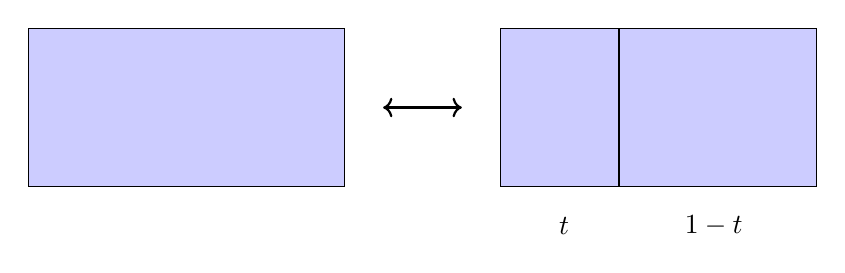
\begin{tikzpicture}
    % 元の容器
    \draw[thick] (0,0) rectangle (4,2);
    \fill[blue!20] (0,0) rectangle (4,2);

    % 分割後の容器
    \draw[thick] (6,0) rectangle (10,2);
    \fill[blue!20] (6,0) rectangle (8,2);
    \fill[blue!20] (8,0) rectangle (10,2);

    % ラベル
    \node at (6.8,-0.5) {$t$};
    \node at (8.7,-0.5) {$1-t$};

    % 矢印
    \draw[<->, thick] (4.5,1) -- (5.5,1);

    % 区切り線
    \draw[thick] (7.5,0) -- (7.5,2);
\end{tikzpicture}
\newpage
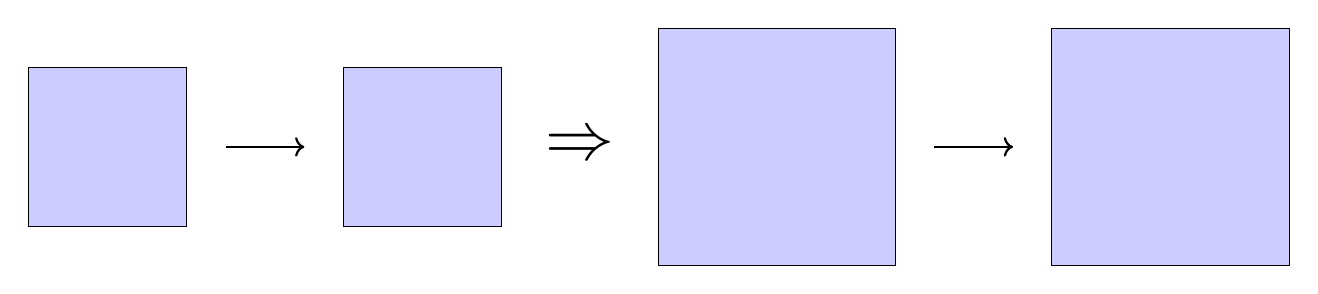
\begin{tikzpicture}
    % 元の容器 A
    \draw[thick] (0,1) rectangle (2,3);
    \fill[blue!20] (0,1) rectangle (2,3);

    % 中間の容器 B
    \draw[thick] (4,1) rectangle (6,3);
    \fill[blue!20] (4,1) rectangle (6,3);

    
    % 最後の容器 tA
    \draw[thick] (8,0.5) rectangle (11,3.5);
    \fill[blue!20] (8,0.5) rectangle (11,3.5);


    % 最後の容器 tB
    \draw[thick] (13,0.5) rectangle (16,3.5);
    \fill[blue!20] (13,0.5) rectangle (16,3.5);

    % 矢印
    \draw[->, thick] (2.5,2) -- (3.5,2);
    \node at (7,2) {\Huge $\Rightarrow$};
    \draw[->, thick] (11.5,2) -- (12.5,2);

\end{tikzpicture}

\newpage
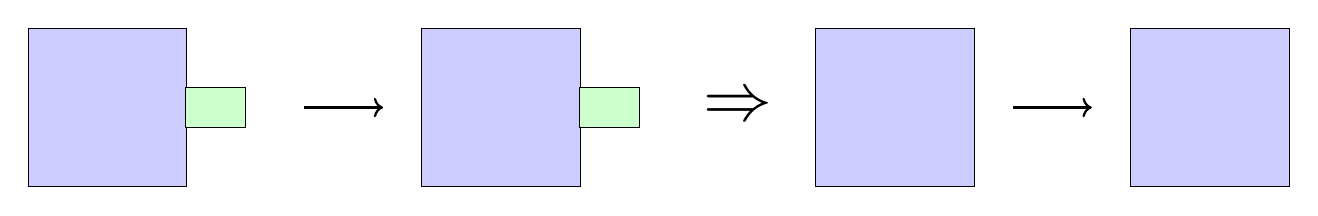
\begin{tikzpicture}
    % 元の容器 A
    \draw[thick] (0,0) rectangle (2,2);
    \fill[blue!20] (0,0) rectangle (2,2);

    % 小さい容器 ε1C
    \draw[thick] (2,0.75) rectangle (2.75,1.25);
    \fill[green!20] (2,0.75) rectangle (2.75,1.25);

    % 中間の容器 B
    \draw[thick] (5,0) rectangle (7,2);
    \fill[blue!20] (5,0) rectangle (7,2);

    % 小さい容器 ε2C
    \draw[thick] (7,0.75) rectangle (7.75,1.25);
    \fill[green!20] (7,0.75) rectangle (7.75,1.25);

    % 最後の容器 A
    \draw[thick] (10,0) rectangle (12,2);
    \fill[blue!20] (10,0) rectangle (12,2);

    % 最後の容器 B
    \draw[thick] (14,0) rectangle (16,2);
    \fill[blue!20] (14,0) rectangle (16,2);

    % 矢印
    \draw[->, thick] (3.5,1) -- (4.5,1);
    \node at (9,1) {\Huge $\Rightarrow$};
    \draw[->, thick] (12.5,1) -- (13.5,1);

\end{tikzpicture}

\newpage

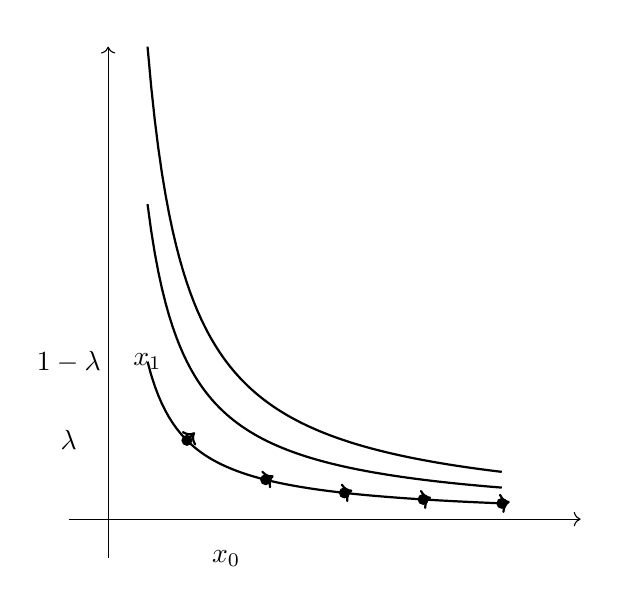
\begin{tikzpicture}
    % 軸の描画
    \draw[->] (-0.5,0) -- (6,0) node[right] {};
    \draw[->] (0,-0.5) -- (0,6) node[above] {};

    % 曲線の描画
    \draw[thick, domain=0.5:5, samples=100] plot (\x, {1/\x});
    \draw[thick, domain=0.5:5, samples=100] plot (\x, {2/\x});
    \draw[thick, domain=0.5:5, samples=100] plot (\x, {3/\x});

    % 点とラベル
    \node at (-0.5,1) {$\lambda$};
    \node at (-0.5,2) {$1-\lambda$};
    \node at (1.5,-0.5) {$x_0$};
    \node at (0.5,2) {$x_1$};

    % ポイントの描画
    \fill (1,1) circle (2pt) node[below left] {};
    \fill (2,0.5) circle (2pt) node[below left] {};
    \fill (3,0.333) circle (2pt) node[below left] {};
    \fill (4,0.25) circle (2pt) node[below left] {};
    \fill (5,0.2) circle (2pt) node[below left] {};
    
    % 矢印
    \draw[->, thick] (1,1) -- (1.1,1.1);
    \draw[->, thick] (2,0.5) -- (2.1,0.55);
    \draw[->, thick] (3,0.333) -- (3.1,0.366);
    \draw[->, thick] (4,0.25) -- (4.1,0.275);
    \draw[->, thick] (5,0.2) -- (5.1,0.22);

\end{tikzpicture}



\end{document}